\documentclass[border=3pt]{standalone}
% Preâmbulo compartilhado pelos diagramas TikZ da aula 8 de IHC (Design de IHC)
\usepackage[T1]{fontenc}
\usepackage[utf8]{inputenc}
\usepackage{lmodern}
\usepackage{amsmath}
\usepackage{xcolor}
\usepackage{tikz}
\usetikzlibrary{arrows.meta,angles,quotes,decorations.pathmorphing,decorations.pathreplacing,calc,
                positioning,shapes.geometric,shapes.misc,backgrounds,fit,
                math}

% Paleta (mesma dos SVGs originais)
% Paleta da disciplina de IHC: acento roxo (#755099), da capa do livro.
% (o nome "dblue" é mantido para não alterar todos os diagramas)
\definecolor{dblue}{HTML}{755099}
\definecolor{dorange}{HTML}{B3541E}
\definecolor{dgreen}{HTML}{4A7C59}
\definecolor{dred}{HTML}{9C4B4B}
\definecolor{dcream}{HTML}{F4F1EA}
\definecolor{dshade}{HTML}{DDD7C9}

% Função gaussiana (não normalizada por padrão de escala visual)
\pgfmathdeclarefunction{gauss}{3}{%
  \pgfmathparse{1/(#3*sqrt(2*pi))*exp(-((#1-#2)^2)/(2*#3^2))}%
}

% Estilos comuns (prefixo d... para não colidir com chaves internas do pgf)
\tikzset{
  >={Stealth[length=2mm]},
  dguide/.style={gray!55, dashed, line width=0.4pt},
  daxis/.style={gray!60, line width=0.7pt, ->},
  dbody/.style={fill=black!3, draw=black!80, line width=1pt},
  dacc/.style={draw=dblue, line width=1pt},
  dlbl/.style={black!55, font=\small},
  dsub/.style={black!45, font=\footnotesize},
  dstate/.style={circle, draw=black!80, fill=dcream, line width=1pt,
                 minimum size=17mm, font=\large, inner sep=1pt},
  dobs/.style={circle, draw=black!80, fill=dshade, line width=1pt,
               minimum size=14mm, font=\large, inner sep=1pt},
  dbox/.style={rounded corners=2pt, draw=black!80, fill=dcream, line width=1pt,
               align=center, inner sep=6pt},
  dop/.style={circle, draw=black!80, fill=white, line width=1pt,
              minimum size=6mm, inner sep=0pt, font=\small},
  dtrans/.style={->, dblue, line width=1pt},
  dmeas/.style={->, dorange, line width=1pt},
  dcurve/.style={line width=1pt, dblue},
  dcurveb/.style={line width=1.4pt, dorange},
}

\begin{document}
\hyphenpenalty=10000 \exhyphenpenalty=10000 \tolerance=9999 \emergencystretch=3em
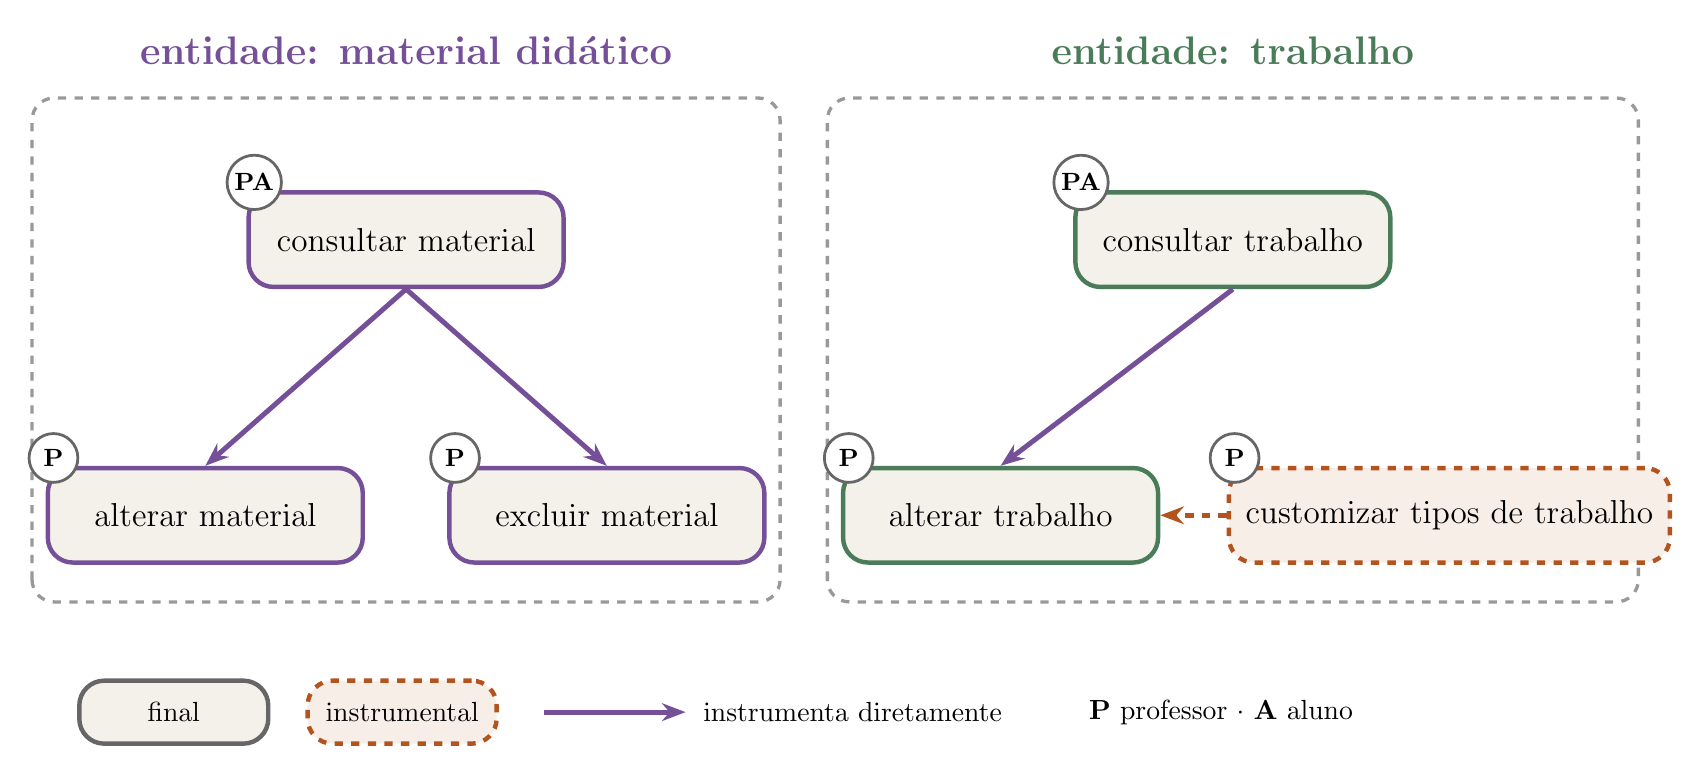
\begin{tikzpicture}[x=1cm,y=1cm]
\tikzset{ob/.style={dbox, rounded corners=9pt, line width=1.6pt, minimum width=4.0cm, minimum height=1.2cm, font=\large},
        inst/.style={dbox, rounded corners=9pt, line width=1.6pt, minimum width=4.0cm, minimum height=1.2cm, font=\large, dashed, fill=dorange!10},
        ba/.style={circle, draw=black!60, fill=white, line width=1pt, font=\small\bfseries, inner sep=1.5pt, minimum size=0.62cm},
        ar/.style={-{Stealth[length=3mm]}, dblue, line width=1.8pt}}
\draw[black!40, dashed, line width=1.2pt, rounded corners=8pt] (-0.3,1.9) rectangle (9.2,8.3);
\node[font=\Large\bfseries, dblue] at (4.45,8.9) {entidade: material didático};
\node[ob, draw=dblue] (c1) at (4.45,6.5) {consultar material};
\node[ob, draw=dblue] (a1) at (1.9,3.0) {alterar material};
\node[ob, draw=dblue] (e1) at (7.0,3.0) {excluir material};
\draw[black!40, dashed, line width=1.2pt, rounded corners=8pt] (9.8,1.9) rectangle (20.1,8.3);
\node[font=\Large\bfseries, dgreen] at (14.95,8.9) {entidade: trabalho};
\node[ob, draw=dgreen] (c2) at (14.95,6.5) {consultar trabalho};
\node[ob, draw=dgreen] (a2) at (12.0,3.0) {alterar trabalho};
\node[inst, draw=dorange] (t2) at (17.7,3.0) {customizar tipos de trabalho};
\node[ba] at ($(c1.north west)+(0.1,0.1)$) {PA}; \node[ba] at ($(a1.north west)+(0.1,0.1)$) {P}; \node[ba] at ($(e1.north west)+(0.1,0.1)$) {P};
\node[ba] at ($(c2.north west)+(0.1,0.1)$) {PA}; \node[ba] at ($(a2.north west)+(0.1,0.1)$) {P}; \node[ba] at ($(t2.north west)+(0.1,0.1)$) {P};
\draw[ar] (c1.south) -- (a1.north);
\draw[ar] (c1.south) -- (e1.north);
\draw[ar] (c2.south) -- (a2.north);
\draw[ar, dorange, dashed] (t2.west) -- (a2.east);
\node[ob, draw=black!60, minimum width=2.4cm, minimum height=0.8cm, font=\normalsize] at (1.5,0.5) {final};
\node[inst, draw=dorange, minimum width=2.4cm, minimum height=0.8cm, font=\normalsize] at (4.4,0.5) {instrumental};
\draw[ar] (6.2,0.5) -- (8.0,0.5); \node[font=\normalsize, anchor=west] at (8.1,0.5) {instrumenta diretamente};
\node[font=\normalsize, anchor=west] at (13.0,0.5) {\textbf{P} professor $\cdot$ \textbf{A} aluno};
\end{tikzpicture}
\end{document}
